\documentclass[10pt]{beamer}

\usepackage[utf8]{inputenc}
\usepackage[T1]{fontenc}
\usepackage{amsmath,amssymb, mathrsfs}
\usepackage{dsfont}\let\mathbb\mathds
\usepackage[english]{babel}
\usepackage[all,dvips]{xy}
\usepackage{tikz-cd}
\usepackage{pgfplots}  

\institute{IBM Research Zurich\\ Université de Rennes 1}
\title{On Oriented Supersingular Isogeny Diffie Hellman}
\author{Pierrick Dartois \\ Under the supervision of Luca De Feo}
\titlegraphic{\includegraphics[width=3.5cm]{logo_IBM.png}\hspace*{1.75cm}~%
   \includegraphics[width=3.5cm]{logo_Rennes1.jpg}
}

\date{September 1 2021}

%\AtBeginSection[]
   %{
   %\begin{frame}
   %\tableofcontents[currentsection]
   %\end{frame}
%}

\usepackage{graphicx} 

\usetheme{Warsaw}

\usepackage{mathtools}

%\theoremstyle{definition}
%\newtheorem{definition}{Definition}

\theoremstyle{plain}
\newtheorem{proposition}{Proposition}
%\newtheorem{lemma}{Lemma}
%\newtheorem{corollary}{Corollary}
%\newtheorem{theorem}{Theorem}

\theoremstyle{definition}
\newtheorem{remark}{Remark}
%\newtheorem{example}{Example}

\usepackage{pgf,tikz}
\usetikzlibrary{arrows}

%To set line spacing
\usepackage{setspace}
% To cross text
\usepackage{ulem}

%macros
\newcommand{\ie}{\emph{i.e.}\ }
\newcommand{\eg}{\emph{e.g.}\ }
\newcommand{\N}{\mathbb{N}}
\newcommand{\Z}{\mathbb{Z}}
\newcommand{\Q}{\mathbb{Q}}
\newcommand{\R}{\mathbb{R}}
\newcommand{\C}{\mathbb{C}}
\newcommand{\K}{\mathbb{K}}
\newcommand{\F}{\mathbb{F}}
\newcommand{\Hc}{\mathbb{H}}
\newcommand{\Lc}{\mathbb{L}}
\newcommand{\M}{\mathbb{M}}
\newcommand{\Pc}{\mathbb{P}}
\newcommand{\A}{\mathbb{A}}
\newcommand{\B}{\mathbb{B}}
\newcommand{\E}{\mathbb{E}}
\newcommand{\V}{\mathbb{V}}
\newcommand{\m}[1]{\mathcal{#1}}
\newcommand{\mA}{\mathcal{A}}
\newcommand{\mB}{\mathcal{B}}
\newcommand{\mC}{\mathcal{C}}
\newcommand{\mP}{\mathcal{P}}
\newcommand{\mK}{\mathcal{K}}
\newcommand{\mL}{\mathcal{L}}
\newcommand{\mE}{\mathcal{E}}
\newcommand{\mD}{\mathcal{D}}
\newcommand{\mF}{\mathcal{F}}
\newcommand{\mO}{\mathcal{O}}
\DeclareMathOperator{\im}{im}
%\renewcommand{\ker}{\mbox{ker}}
%\renewcommand{\dim}{\mbox{dim}}
%\renewcommand{\deg}{\mbox{deg}}
\renewcommand{\i}[2]{\left\llbracket #1~;~#2\right\rrbracket}
\renewcommand{\(}{\left(}
\renewcommand{\)}{\right)}
\renewcommand{\P}{\mathbb{P}}
%commandes de Quentin
%\newcommand{\F}[1]{\mathbb{F}_{#1}}
\newcommand{\Fp}[1]{\mathbb{F}_{p^{#1}}}
\newcommand{\db}[1]{\mathbb{#1}}
\newcommand{\id}{\mbox{id}}
\newcommand{\mf}[1]{\mathfrak{#1}}
\newcommand{\mfm}{\mathfrak{m}}
\newcommand{\mfn}{\mathfrak{n}}
\newcommand{\mfp}{\mathfrak{p}}
\newcommand{\mfq}{\mathfrak{q}}
\DeclareMathOperator{\Spec}{Spec}
\DeclareMathOperator{\Proj}{Proj}
\DeclareMathOperator{\Hom}{Hom}
\DeclareMathOperator{\End}{End}
\DeclareMathOperator{\Aut}{Aut}
\DeclareMathOperator{\Tr}{Tr}
\DeclareMathOperator{\disc}{disc}
\DeclareMathOperator{\Cl}{Cl}
\let\SS\relax
\DeclareMathOperator{\SS}{SS}
\DeclareMathOperator{\Ell}{Ell}
%\DeclareMathOperator{\mod}{mod}
\DeclareMathOperator{\Gal}{Gal}
\DeclareMathOperator{\nrd}{nrd}
\DeclareMathOperator{\Vol}{Vol}
\DeclareMathOperator{\Covol}{Covol}
\DeclareMathOperator{\lcm}{lcm}
\DeclareMathOperator{\ProjEval}{ProjEval}
\DeclareMathOperator{\Char}{char}%\char already taken
\DeclareMathOperator{\DL}{DL}
\DeclareMathOperator{\argmax}{argmax}

\newcommand{\leftmapsto}{\leftarrow\!\shortmid}
\newcommand{\longleftmapsto}{\longleftarrow\!\shortmid}
\renewcommand{\vec}[1]{\mathbf{#1}}


\begin{document}

\begin{frame}
\titlepage
\end{frame}

\begin{frame}
\tableofcontents
\end{frame}

\section{Introduction}

\subsection{Presentation of IBM Research}

\begin{frame}
% 3000 poeple in 12 countries 
\textbf{Key research areas in IBM Research}

\begin{columns}[t]
\column{.5\textwidth}
\begin{figure}
\includegraphics[width=3.5cm]
{science_and_technology.png} 

Science and Technology

\vspace{0.1cm}

{\setstretch{0.5} {\footnotesize Quantum computing, nanotechnologies, semi-conductors, electronics,  green technologies...}\\}
\vspace{0.3cm}


\includegraphics[width=3.5cm]
{security.jpg} 

Security

\vspace{0.1cm}

{\setstretch{0.5} {\footnotesize Post-quantum cryptography, blockchain, cybersecurity, identity and data governance...}\\}
\end{figure}


\column{.5\textwidth}

\begin{figure}
\includegraphics[width=3.5cm]
{cloud_and_AI.png} 

Cloud and AI

\vspace{0.1cm}

{\setstretch{0.5}{\footnotesize Machine learning, hardware technologies for storage, memory and processing in the cloud...}\\}

\vspace{0.3cm}

\includegraphics[width=3.5cm]
{cognitive_computing.jpg}

Cognitive computing

\vspace{0.1cm}

{\setstretch{0.5}{\footnotesize Computational biology and medicine, supercomputing, predictive maintenance...}\\}
\end{figure}
\end{columns}

\end{frame}

\subsection{Contextualization of OSIDH}

\subsubsection{Post quantum and isogeny based cryptography}

\begin{frame}
\textbf{Quantum computers are a threat to current cryptography}

\begin{itemize}
\item Shor's algorithm (1995) can compute discrete logarithms and factor integers on a quantum computer.

\item All current public key cryptography based on these problems may become unsafe (\sout{RSA} and \sout{El Gamal}).
\end{itemize}

\begin{columns}[t]
\column{.3\textwidth}

\begin{figure}
\includegraphics[width=3cm]{quantum_computer.png} 

\end{figure}


\column{.7\textwidth}

\begin{figure}
\includegraphics[width=6cm]{hammer.jpeg} 
\end{figure}

\end{columns}

\end{frame}



\begin{frame}
\textbf{Isogeny based cryptography in the NIST competition}

\begin{columns}[t]
\column{.5\textwidth}

\begin{figure}
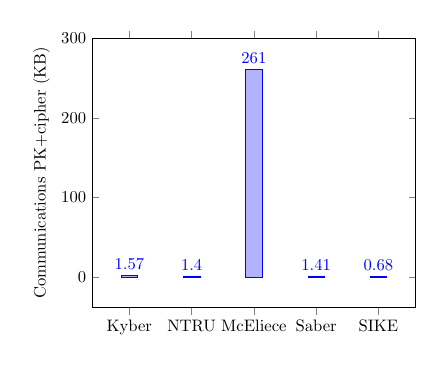
\begin{tikzpicture}[scale=0.6]
  
\begin{axis}  
[  
    ybar,  
    enlargelimits=0.15,  
    ylabel={Communications PK+cipher (KB)}, % the ylabel must precede a # symbol.  
    %xlabel={},  
    symbolic x coords={Kyber, NTRU, McEliece, Saber, SIKE}, % these are the specification of coordinates on the x-axis.  
    xtick=data,  
     nodes near coords, % this command is used to mention the y-axis points on the top of the particular bar.  
    nodes near coords align={vertical},  
    ]  
\addplot coordinates {(Kyber,1.568) (NTRU,1.398) (McEliece,261) (Saber,1.408) (SIKE,0.676) };  
  
\end{axis}  
\end{tikzpicture} 

\caption{Total size of public key and cipher in kilo bytes of 5 NIST round 3 KEM candidates.}
\end{figure}

\column{.5\textwidth}

\begin{figure}
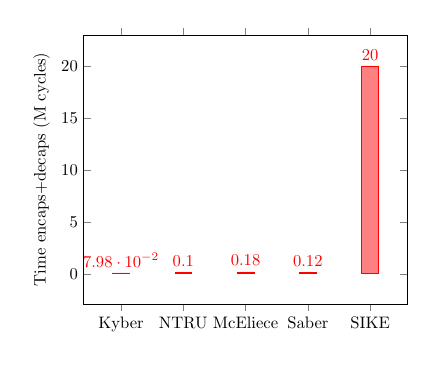
\begin{tikzpicture}[scale=0.6]
  
\begin{axis}  
[  
    ybar,  
    enlargelimits=0.15,  
    ylabel={Time encaps+decaps (M cycles)}, % the ylabel must precede a # symbol.  
    %xlabel={},  
    symbolic x coords={Kyber, NTRU, McEliece, Saber, SIKE}, % these are the specification of coordinates on the x-axis.  
    xtick=data,  
     nodes near coords, % this command is used to mention the y-axis points on the top of the particular bar.  
    nodes near coords align={vertical},  
    ]  
\addplot[color=red,fill=red!50] coordinates {(Kyber,0.079772) (NTRU,0.101357) (McEliece,0.179095) (Saber,0.124) (SIKE,20) };  
  
\end{axis}  
\end{tikzpicture}

\caption{Total time performance (encapsulation and decapsulation) in mega cycles of 5 NIST round 3 KEM candidates.}
\end{figure}

\end{columns}

\end{frame}

\subsubsection{Diffie Hellman key-exchange}

%Show cryptographic group action, Couveignes cryptosystem, CSIDH, OSIDH.

\section{Introduction to OSIDH}

\subsection{Orientations}

\subsection{Oriented supersingular isogeny graphs}

\subsection{The ideal class group action}

\subsection{Chains and ladders}

\section{The OSIDH protocol}

\subsection{A broken naive Diffie Hellman protocol}

\subsection{Why is it broken?}

\subsection{A fixed Diffie Hellman protocol}

\section{Cryptanalysis of OSIDH}

\subsection{Recovering the chain with oriented endomorphisms}

\subsection{A lattice reduction to find oriented endomorphisms}

\subsection{Implementation of our attack}

\subsection{Countermeasures}

\section{Conclusion}

\end{document}